\documentclass{article}
\author{
  Torrent Gorjon, Xavier\\
  \texttt{Xavier.TorrentGorjon@os3.nl}
}
\title{Protecting against relay attacks forging increased distance reports}

\usepackage{graphicx}
\usepackage[backend=bibtex]{biblatex}

\setcounter{secnumdepth}{4}


\bibliography{references}


\begin{document}


\begin{titlepage}
\center
\textsc{}\\[1cm]
\textsc{\LARGE Universiteit van Amsterdam}\\[1.5cm]

\textsc{\Large Research Project I}\\[0.5cm]

\textsc{\Huge Protecting against relay\\[0cm] attacks forging increased\\[0.5cm] distance reports}\\[1.5cm]


\includegraphics[scale=1]{images/uva.png}\\[1cm]

\begin{minipage}{0.5 \textwidth}
\begin{center} \large
Xavier Torrent Gorj\'{o}n\\
\emph{Xavier.TorrentGorjon@os3.nl}\\[0.5cm]
\end{center}
\end{minipage}\\[2cm]
{\large \today} 


\end{titlepage}


\newpage


\renewcommand{\abstractname}{\Large Abstract}
\begin{abstract}
For a long time, distance-bounding protocols have been an extensive research topic due to their usefulness as a security feature for systems that assume a specific proximity between parties, such as Passive Keyless Entry Systems (PKES) for cars. However, we did not find on the current literature any attempts to use these protocols to prevent relay attacks forging increased distance reports.

This project first proposes a variety of scenarios, in which the involved devices use distance-bounding protocols to perform distance checks between themselves. Relay attacks that attempt to fake increased distance reports between these devices will be studied, and a discussion of the motivation these attacks might have, as well as their consequences, will be provided.

Afterwards, available systems that could be used instead of distance bounding protocols will be reviewed. In particular, the analysis will focus on Global Positioning System (GPS), Inertial Navigation System (INS) and Radio Detecting and Ranging (RADAR) systems. This study will aim to justify developing solutions based on the current distance-bounding protocols, providing an insight on the limitations of these other systems for these purposes.

Some low-cost, easy-to-implement enhancements on the distance-bounding protocols will be proposed, which diminish the success chances of these relay attacks against systems using these protocols.
\end{abstract}

{\bf Keywords --- Relay attack, distance-bounding protocol} 

\newpage

\section*{Glossary}
\addtocounter{section}{0}

\begin{description}
  \item[ACS] Access Control System: Systems that use authentication mechanisms to validate the access to resources.
  \item[GPS] Global Positioning System: Navigation system based on satellite communication maintained by the United States government.
  \item[INS] Inertial Navigation System: Navigation system that keeps track of the route used by an object to have awareness of its location.
  \item[LIDAR] Light Detection and Ranging: Object-detection system based on laser.
  \item[MANET] Mobile Ad-Hoc Network: A network of independent devices deployed for a specific purpose.
  \item[PKES] Passive Keyless Entry Systems: A type of access control, usually used in cars, that features the possibility of automatically opening doors without need of interaction from the user.
  \item[RADAR] Radio Detection and Ranging: Object-detection system based on radio waves.
  \item[RCS] Radar Cross Section: Signature of an object on a RADAR system.
  \item[ToF] Time-of-Flight: Measurement on the time required to receive a signal response from another party after a signal is sent.
\end{description}

\newpage



\tableofcontents





\newpage








\section{Introduction}
\label{sec:introduction}

Communications between machines face many challenges when the transmitted information needs to be protected. Most communications can prove to be valuable attack points for third parties that want to recover, modify, block or otherwise manipulate the original message for personal profit. Part of these attacks can be prevented by using end-to-end encryption and signature of the data. However, relay attacks cannot be prevented just by using cryptographic algorithms.\\

Relay attacks consist of the mere reception and replay of information. Although at first this might seem harmless, many systems become vulnerable if that relaying of information is not noticed. One scenario that can be used as an example of the threat these attacks represent are Access Control Systems (ACS), in which a device is used to prove that a user is within a certain distance from a validator through a challenge-response protocol. On unprotected implementations of these access control systems, an attacker can relay the challenge from the validator to a valid user who is not in range and relay its answer back to the validator, effectively bypassing distance validation. Practical attacks on this kind of systems have been demonstrated in various studies \cite{francillon2011relay, francis2010practical, hancke2005practical, markantonakis2012practical}.\\

This paper, however, will study attacks that are not related to proximity-checking systems. Distance-bounding protocols are already an effective solution for ACS and other systems that validate the proximity of a user before performing operations, and are only limited by the specifications of the systems that need to implement such protocols. Nonetheless, we did not find, in the current literature, attempts to use distance-bounding protocols to prevent forged increased distance reports, although this was an acknowledged issue on the distance-bounding studies. We intend to show that these attacks can be a menace, and propose solutions to prevent them.\\

This document is structured as follows: in Section \ref{sec:relatedwork} we review the literature used in this project. Section \ref{sec:researchquestions} presents a detailed explanation on the research questions this project aims to answer. Following in Section \ref{sec:methodology}, an explanation of the methodology used in this study is provided. Section \ref{sec:dbandalternative} discusses the actual results from our initial investigation, including an explanation on how distance-bounding protocols work and a study of alternative systems that could be used as countermeasures to the discussed relay attacks. Proposal of various scenarios in which relay attacks forging increased distance reports could be used are presented in Section \ref{sec:attackfeasibility}. Some solutions based on the current distance-bounding protocols will be proposed on Section \ref{sec:prevention}, analysing the level of protection they provide, as well as the feasibility and cost of using them. Conclusions are gathered in Section \ref{sec:conclusions}, which includes a review and a discussion of the obtained results.\\







\section{Related Work}
\label{sec:relatedwork}

There is much literature available presenting solutions to distance bounding problems \cite{brands1994distance, rasmussen2010realization, tu2007rfid}. All of these studies are part of a constant iteration to improve the protocols. As new attacks emerge against distance bounding protocols, new studies are published to fix the deficiencies of the previous work. This project will use these previously mentioned studies as a basis for the solutions against the studied relay attacks. Even the older documents still prove to be useful, as they can be used as an introduction to the topic and to understand how this field has evolved.\\

There are also many practical studies in the field of distance bounding, which aim to test the vulnerabilities on real applications \cite{vandenbreekel2014relay, francillon2011relay, francis2010practical, hancke2005practical, markantonakis2012practical}. Although all these refer to forging decreased distance reports and they are not directly used in our research, they have been useful as a starting point.\\

This project will assume certain conditions for the studied attacks. Some assumptions and justifications will be required on the investigation, based on the characteristics of GPS signals. Many studies focus on the feasibility of intentional attacks against GPS systems \cite{jafarnia2012gps, warner2003gps, wen2005countermeasures}. These studies conclude that, even though spoofing is hard with the solutions they propose, it is not impossible. With this premise, the goal will be to develop countermeasures against relay attacks without relying on GPS signals.\\

In a similar way to GPS signals, other systems such as RADAR detection \cite{cadirci2009rf} and Inertial Navigation Systems (INS) \cite{patent:4085440} could arguably be used to prevent relay attacks. Using these information sources \cite{cadirci2009rf, patent:4085440}, we explain why neither of these systems are reliable, reaffirming the need of a modified distance bounding protocol that is not vulnerable to relay attacks.\\

Finally, this study is closely related to the field of MANETs (Mobile Ad-hoc NETworks), and as such, literature available on this topic is of our interest. In particular, wormhole attacks \cite{goyal2010literature, hu2006wormhole, maheshwari2007detecting} are a specific type of relay attack that, while being different than the ones we will study in this document, provide valuable insight to our investigation.\\














\section{Research Questions}
\label{sec:researchquestions}

As seen in Section \ref{sec:relatedwork}, in the current literature we did not find proposals to fight the subset of relay attacks that attempt to fake increased distance reports between legitimate parties. This project will first study the difficulty of performing these attacks. Therefore, our first research question will be:\\

\emph{Feasibility of forged increased distance report relay attacks}\\

We first present a detailed description of various distance-bounding protocols using different kinds of approaches to check distances between parties, explaining how do they work and their limitations.\\

Following the protocol discussion, we explore a number of real world scenarios that could use these protocols. Some theoretical attacks on these systems will be proposed, discussing their feasibility and consequences on the studied systems. This analysis is necessary, as the first goal of this project is to prove that these attacks can be dangerous, given the right circumstances. The proposed scenarios are diverse, both in context and properties of the systems involved, implying that the possible solutions for one case might not suit others, especially when considering hardware limitations and economic costs.\\

After the discussion on the study cases, an evaluation of other systems that could be used to prevent those attacks will follow. This evaluation will include GPS location, INS, as well as RADAR detection. The investigation on GPS and INS systems will focus on their usability as positioning systems, while the study of RADAR will evaluate its usefulness when attempting to physically detect attackers.\\

If the results from this research determine that these attacks can pose a threat and that the alternative systems are not enough to prevent them, we will consider a second research question:\\

\emph{Preventing forged increased distance report relay attacks}\\

This second research question will focus on providing solutions to the issues stated on the first. Original distance-bounding protocols used to perform upper-bound distance checking can rely on the speed of light to completely prevent relay attacks faking closer distances between parties. Attacks forging increased distance reports, however, are performed by delaying the original signal, which means that the physical limitation of the speed of light cannot be used to prevent them. From this initial consideration we expect that it will not be possible to provide a solution that completely blocks these attacks. Nevertheless, it may be possible to find countermeasures that greatly reduce the chances of successfully performing these attacks.\\








\section{Methodology}
\label{sec:methodology}

This project will be a theoretical research on the current distance-bounding protocols, and their inability to detect increased distance reports. We intend to expose the limitations of these protocols on specific real world scenarios, and ultimately offer solutions to them.\\

First, we provide a review of the available literature about distance-bounding protocols, in order to determine which of them is best suited for our research. A discussion of alternative systems that could be used to prevent these attacks will be provided as well.\\

Following the distance-bounding protocols description, this document will propose systems that could be vulnerable to these attacks, reviewing the difficulty of these attacks and the consequences these attacks might have. In particular, the focus will be on autonomous cars and drones. These scenarios will be the basis for our research.\\

At the last part of the paper, variation proposals of the distance-bounding protocols will be provided, in order to effectively reduce the threat these attacks pose. We discuss the increase in security these solutions achieve, as well as evaluating the feasibility of implementing them on our study cases.\\













\section{Distance-bounding protocols and alternative systems}
\label{sec:dbandalternative}

In this section, we discuss distance-bounding protocols, as well as GPS and INS location systems and RADAR detection. All of them are relevant topics to our research. First, an explanation on the current distance bounding protocols will be provided, as they are used as a starting point for our research. Afterwards, GPS and INS systems will be evaluated, explaining why the studied systems shouldn't rely completely on them, hence the need to develop more powerful distance-bounding protocols. Lastly, we discuss the possibility of using RADAR detection to fight the proposed attacks.\\

\subsection{Distance-bounding protocols}

Distance-bounding protocols were developed as a countermeasure to relay attacks that attempt to fool systems that validate the proximity of a user to a validation point. Common scenarios of these applications are found in ACS, such as smartcards to access buildings or cars using PKES.\\

These distance-bounding protocols try to use properties of the systems involved in the communications (such as signal intensity or message Time-of-Flight (ToF)) to validate the proximity of users. Based on the previous studies available \cite{capkun2006secure}, we will proceed to briefly discuss these methods:\\

\begin{description}
  \item[Signal Intensity] Signal intensity protocols try to achieve proper location of other nodes by measuring the received signal strength. Previous work available in the public literature\cite{seshadri2005bayesian} proves the usefulness of this location system. Even though attacks on these systems are hard to perform \cite{sheng2008detecting}, the majority of defences against them rely on anomaly detection. The reliability of these systems can be decreased in heavily adverse situations, and the ToF methods discussed next provide a higher degree of security.\\
  \item[Ultrasound ToF] Ultrasound ToF measures the round-trip time of messages sent and received from the parties measuring the distance between them. This does not depend on the signal strength for the measurement, although ultrasound-based ToF has the latent vulnerability that other methods, such as radio frequency or optical wires, attackers can surpass the speed of the ultrasound communication, effectively being able to relay information faster than the legitimate infrastructure\cite{capkun2006secure}.\\
  \item[Radio ToF] Radio-based ToF uses the same method as ultrasound ToF to perform the distance check. The key of the success of this method is that the information transmitted travels at speeds near the speed of light, meaning there is no physical way to fake one node is closer than it really is. Practical studies on this method \cite{rasmussen2010realization} developed hardware that can perform the operations required under 1ns, meaning that the maximum theoretical distance an attacker can shorten its reported distance is under 15cm.\\\
\end{description}

In this project we use Radio ToF distance-bounding as a basis for our work, as it is proven to be the most secure and reliable method. In particular, the implementation that will be assumed to be used, will be the one described in \cite{rasmussen2010realization}, as it is the most recent and secure developed protocol. This distance-bounding protocol is based purely on analog signals, avoiding the time required to convert analog signals into digital signals. A graphical diagram of the communication channels can be found in Figure \ref{fig:dbounding1} and, following next, there is a description of the inner workings of the system:\\



\begin{enumerate}
  \item First, both validator $V$ and prover $P$ exchange a nonce $N$. This can be done on-the-fly or before the system starts.
  \item When it is necessary to verify the current distance of the two parties, $V$ starts sending challenging bits $C_{n}$ to $P$.
  \item For every bit $C_{i}$ received, $P$ sends back a response in the form of $C_{i}+N_{i}$. The answer is done by sending the bit $C_{i}$ through one of the two communication channels for the challenge answers, while the bit $N_{i}$ is encoded implicitly in the form of which answer channel was selected. For example, if the current nonce bit $N_{i}$ is $0$, the $C_{i}$ answer would be sent using the first channel, whereas if its value of $N_{i}$ was $1$, the second channel would be used.
  \item Step 3 is repeated $n$ times. The chances of an attacker faking one of the response transmissions is $\frac{1}{2}$, but after $n$ times of repeating this operation, the possibility of an attacker faking the whole procedure goes down to $\frac{1}{2\textsuperscript{n}}$. 
  \item Finally, $V$ can calculate the mean value of all the challenge-response ToF, effectively obtaining the distance between him and $P$.
\end{enumerate}




\begin{figure}[h!]
  \centering
    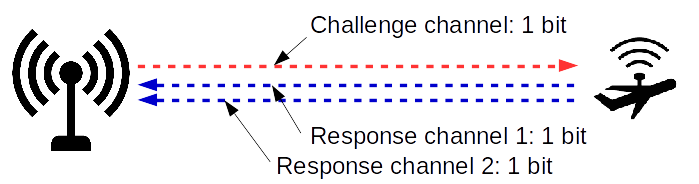
\includegraphics[width=1\textwidth]{images/dbounding.png}
  \caption{Channels in the distance-bounding Protocol proposed by \citeauthor{rasmussen2010realization}.}
  \label{fig:dbounding1}
\end{figure}



However, although this protocol alone can prevent relay attacks attempting to forge decreased distances between the legitimate parties, it is not enough to fight attacks that forge an increase on the real distance, and this will be the main focus of our research.\\



\subsection{GPS location}

It could be argued that GPS location can be used to prevent the attacks that we will discuss on the next subsection. However, GPS signals have their own weaknesses both with and without presence of adversaries.\\

In settings without adversaries, GPS positioning cannot be reliably used indoors or underground, and sometimes the presence of tall buildings or structures nearby is enough to disrupt its data.\\

Considering scenarios with one or multiple adversaries, even though there are many countermeasures to prevent attacks against GPS positioning \cite{warner2003gps, wen2005countermeasures, jafarnia2012gps}, they do not provide complete security, similar to the Signal Intensity location protocol.\\

Due to these problems, the U.S. government actually recommends to always have backup systems for GPS and suggests to never rely entirely on it\footnote{\url{http://www.gps.gov/support/faq/#jamming}}. Based on these premises we will assume that GPS is not a part of our system, or that we cannot rely on it.\\

\subsection{Inertial Navigation System}

Inertial Navigation Systems are devices used to provide machines a sense of self-awareness of their current position, based on their initial position and the chosen routes, by using accelerometers and gyroscopes. These systems could be relevant for this research, as they share the same \emph{relative positioning} focus, staying independent from third party sensors.\\

INS hardware cannot realistically provide an accuracy below $5m$ of error after $60$ seconds of operation \cite{woodman2007introduction}. In an environment with multiple nodes using this system, this means that after $60$ seconds, the location detection between two nodes could be as biased as $10m$. This also limits its usability as a stand-alone positioning system, as the error will only grow larger as time progresses.\\

Although INS accuracy is rapidly improving over the years, at the moment is not a viable solution or countermeasure to our problem.\\

\subsection{RADAR detection}

One way to protect against this kind attack could be by attempting to physically detect the attacker that is attempting to perform the relaying of messages. If an unidentified object is detected between the parties and it is confirmed that it does not belong to the system, security measures could be taken to prevent such relay attacks.\\

However, recent studies as the one by \citeauthor{cadirci2009rf} in \cite{cadirci2009rf}, state that Radar Cross Section\footnote{\url{http://www.microwaves101.com/encyclopedia/Navy handbook/4.11 Radar Cross-Section (RCS).pdf}} (RCS), a measurement used to rate the ability to reflect radio waves by an object, can be heavily decreased by employing proper techniques such as the usage of special materials, radiowave-absorbing paint and specific shapes that minimize and disperse radio reflection.\\

As a real world example, the first operational aircraft designed to employ advanced stealth technology, the Lockheed F-117 Nighthawk from the United States Air Force, with a wingspan and a length of $13.20m$ and $20m$ respectively\footnote{\url{http://www.fighter-planes.com/info/f117_nighthawk.htm}}, has a RCS signature of $0.025m^2$, which is similar to that of a bird\cite{cadirci2009rf}.\\

In the attack scenarios proposed in Section \ref{sec:results}, flying drones would be the most versatile device to perform the attacks. Considering these drones can be considerably smaller than these aircraft (depending on the situation, the used drone could be shorter than $1m$ in length, height and width), it is easy to foresee that they would be almost invisible to radar systems. If the attack scenario does not require the attacker to fly at relative high speeds, its RCS signature could be further decreased by designing an attack drone with a shape specifically made to absorb radar waves.\\

We therefore conclude that, in the current state of stealth and anti-stealth technologies, RADAR detection would not be a strong countermeasure to prevent against that kind of attacks.\\







































\section{Feasibility of forged increased distance report relay attacks}
\label{sec:attackfeasibility}

The theoretical attack we propose relies on the fact that the discussed protocols regarding distance bounding on the available literature do not prevent relay attacks that report an increased distance between two legitimate parties.\\

The basics of the attack are easy to understand. Assume two parties are communicating using a transmitter-receiver model, that is, one of them is actively reporting its position to the other, using the distance-bounding protocol. At some point, an attacker seizes a position between them and starts disrupting the communication between them, either by attempting to block the communication or by jamming its frequency range. At the same time, he starts recording the information and resending it to the receiver node, adding a brief delay on it. Figure \ref{fig:attackexample1} provides a graphical description of the problem. The effectiveness of this attack can be increased by having multiple malicious nodes attempting to block the original signal.\\

\begin{figure}[h!]
  \centering
    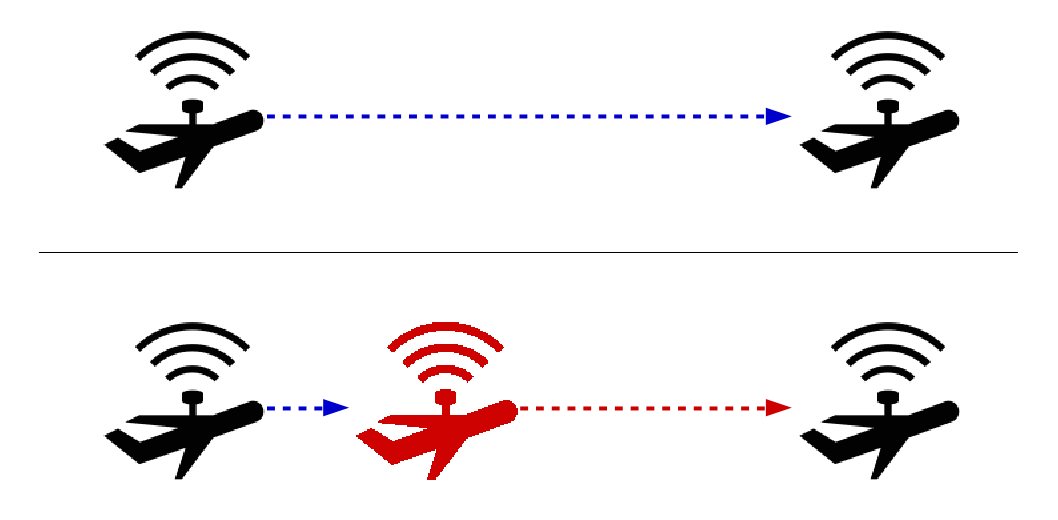
\includegraphics[width=0.8\textwidth]{images/attack1.png}
  \caption{Regular communication versus block and relay attack.}
  \label{fig:attackexample1}
\end{figure}

Many systems use these distance reporting protocols for their pathing decisions. This kind of attack could cause unexpected behaviour on the systems, effectively altering their original desired outcome.\\

Such attacks are difficult to perform in practice, as they require relaying and jamming communications at the same time. Appropriate timing on the relay and some degree of knowledge about the system are also required to successfully perform an attack. However, this could be done in theory.\\

Following next, we will discuss some real world applications that may be interesting for this research.\\

\subsection{First example of real world attack: Autonomous cars}

Autonomous driving is a topic that is receiving a lot of attention by many researchers around the globe in recent years. The variety and quantity of studies on this field \cite{franke1999autonomous,continentalautonomous,levinsontowards,geiger2012we}, prove its relevance as an interesting subject from the point of view of computer vision and location systems.\\

These autonomous cars use multiple systems to check and validate their position and the layout of the surrounding area. Usually these systems include a subset of GPS location, lasers, radars and computer vision systems \cite{continentalautonomous,levinsontowards}.\\

Distance bounding protocols do not seem to be an active part of these systems, although they could be useful. First of all, the most obvious utility would be to provide an additional security layer to the system, providing additional means to locate other vehicles in normal conditions, or as a backup system in case other devices fail. Secondly, this feature could be used as well to detect pedestrians in a future if devices such as mobile phones were adapted for this purpose.\\

Autonomously driving vehicles could also use distance bounding protocols to perform distance verification of specific targets. The distance bounding protocols developed in  \cite{rasmussen2010realization, capkun2006secure} can be used to check the distance with specific targets. This is interesting in this environment as in a high traffic road it is difficult to keep track of other specific vehicles through the use of Light Detection and Ranging (LIDAR) or computer vision system. This functionality could be used, for example, to have a car follow another without knowing the route beforehand.\\

Although the introduction of these distance bounding protocols on autonomous cars could prove to be useful for these purposes, it would also add a vulnerability in the form of the previously mentioned reported distance increase relay attacks.\\


\subsection{Second example of real world attack: Drone MANETs}

In the recent years there has been a huge increase on the interest towards drones\footnote{\url{http://www.google.com/trends/explore#q=drone}}, due the emergence of topics such as Amazon Prime delivery drones (Figure \ref{fig:amazondrone} or the usage of unmanned aircraft by the US military.\\


\begin{figure}[h!]
  \centering
    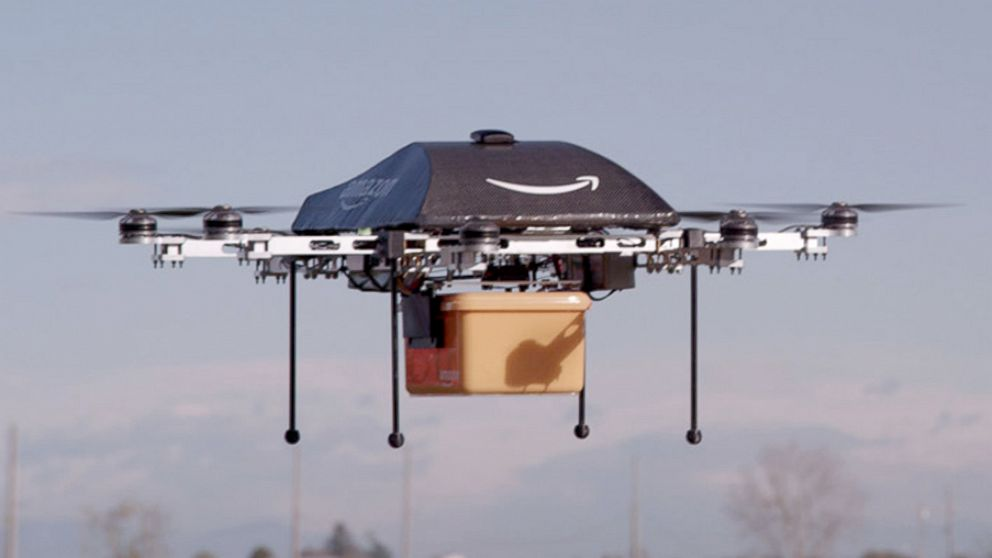
\includegraphics[width=0.6\textwidth]{images/amazonprimedrone.png}
  \caption{Amazon Prime delivery drone carrying a package.}
  \label{fig:amazondrone}
\end{figure}

It is safe to foresee that the usage of drones will only grow on the upcoming years due their ability to decrease costs and improve the performance of systems currently manned by humans. We present two scenarios on which the use of drones can be interesting and how can they be affected by the discussed relay attacks.\\

\begin{description}
  \item[Cooperative working drones] Taking as an example the Amazon Prime delivery drones, we can discuss the possibility of having multiple drones working in groups. One interesting scenario is the case of multiple drones carrying a larger package. For a company trying to keep expenses low, it would make sense to use multiple drones that can work cooperatively in different situations rather than having drones of various sizes for each type of package. In this situation, an attacker could try to attack that system by faking some drone's distance reports to the others, which may force the drones to change positions and loose equilibrium, eventually crashing.\\
 
  A relay attack on this platform could make more sense than just attempting to shut down the drones to achieve the same goal, as it would be extremely difficult to prove that a relay attack took place by checking the logs of the crashed drones. This could lead to a reputation loss for the delivery company, as their system would be seen as unreliable by the customers. Even though this kind of delivery platform has not been deployed yet duelegal constraints, it may start to be available at some point in 2015\footnote{\url{http://abcnews.go.com/Technology/amazon-prime-air-delivery-drones-arrive-early-2015/story?id=21064960}}.\\
  
  
  \item[Area surveillance drones] Another common use of drone MANETs is to perform area surveillance. This case has both civilian and military applications. Civilian use cases range from searching missing people to area mapping, while military uses usually imply area reconnaissance searching for possible threats or targets.\\
  
  In this particular situation where a group of drones is checking a zone, an attacker could attempt to interfere in the reported distances. This could cause the drones to believe they are further apart between themselves than what they really are. Under these circumstances, they could decide to get closer together so they do not leave zones unchecked between them, which would inevitably cause a reduction on the covered area. Figure \ref{fig:attackexample2} represents an example of this attack.\\
  
  \begin{figure}[h!]
  \centering
    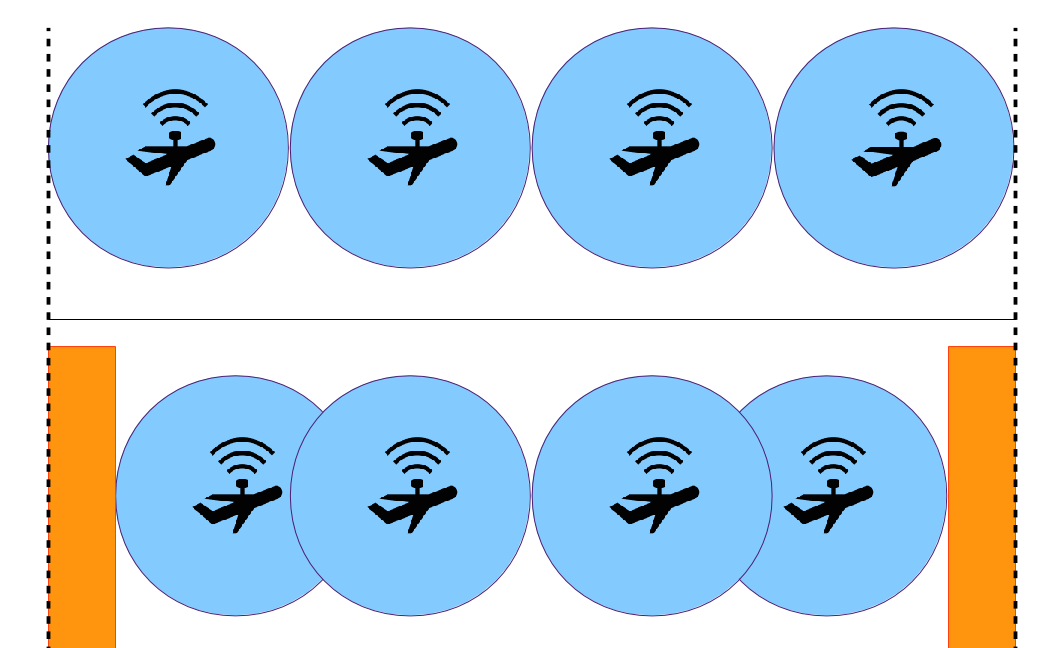
\includegraphics[width=0.8\textwidth]{images/attack2.png}
  \caption{Example of the proposed attack. On the first case, the four drones manage to explore all the expected area (marked with trailing dots). On the second, the marked zones on the sides represent the resulting unchecked area as a consequence of this attack.}
  \label{fig:attackexample2}
\end{figure}

This attack might prove considerably difficult to perform, but can have catastrophic consequences if successful. Unlike the attack on cooperative drones, distance is less of a restriction here, but in this case the attack requires a much deeper knowledge of the attacked system.\\

\end{description}



















\section{Preventing forged increased distance report relay attacks}
\label{sec:prevention}

In this section some countermeasures to the studied relay attacks are proposed. These solutions can stack with one another and, in fact, it is recommended to do so, as each one of them provides an additional layer of security.\\

These solutions do not need new protocols or hardware, and instead rely on the replication and addition of redundancy to provide protection against the fake increased distance reports. This means that the systems discussed on the first research question could implement these with minimal modifications.\\

\subsection{Introducing behaviour verification}

Nowadays storage is hardly a limitation for systems, as the price, size and weight of these components have decreased to the point where multiple gigabytes of information can be stored in inexpensive memories that have the size of a screw.\\

Therefore, storing information on the device about the recent location of one or multiple parties is feasible. Uncoordinated attacks would be prevented with this feature, although it does little to protect against carefully planned ones. All location systems must allow some degree of variation on the measurements, as there may be many reasons for a slight delay in a communication. By successfully using that error margin, an attacker could still attempt to fake distance reports increasingly over a period of time.\\



\subsection{Utilize multiple distance-bounding signals}

Historically, distance-bounding protocols are used to validate an upper-bound distance between a prover and a validating station. As such, the exact location of a prover is not required, only its distance to the validating station matters (that is, check if the prover is within a certain radius of the prover in a 2D scenario, or a sphere in a 3D scenario).\\

If the nodes using distance-bounding protocols are large enough, multiple distance-bounding antennas can be used so that not only the distance from another node is known, but also its approximate location on the 3D space.\\

By using this triangulation system, attackers need to temper the communication between several antennas at the same time. Coupled with the behaviour verification solution, it becomes easier to detect relay attacks. For an attacker it is still easy to produce fake distance reporting positions on the same vector of the legitimate prover, but it becomes increasingly difficult to fake positions that diverge from that line.\\

Figure \ref{fig:attackexample3} provides a graphical explanation of this defence mechanism. An attacker cannot make the left drone believe that the legitimate drone is inside the circle area, due the original distance-bounding protocol features. With this method an attacker can still fake a position in the darker area with relative ease, but faking a position outside from it becomes increasingly difficult as multiple distance reports have to be taken into account, and a deviation on any of them could end with the checking drone detecting inconsistency in the received data.\\

  \begin{figure}[h!]
  \centering
    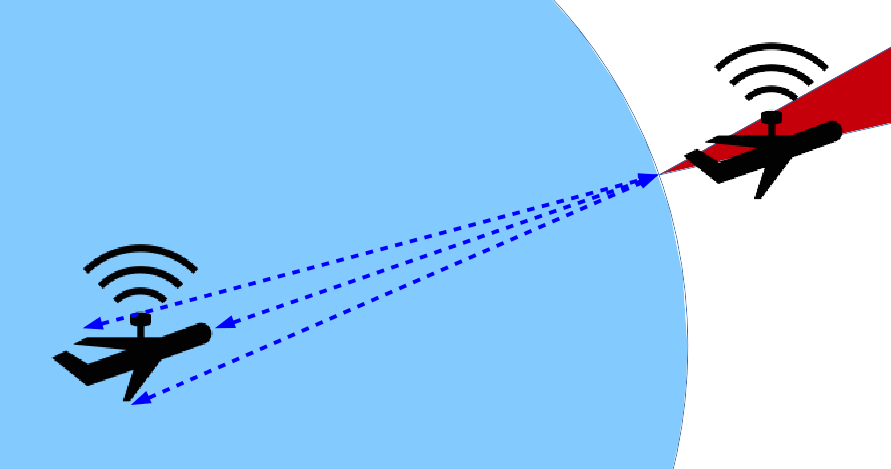
\includegraphics[width=0.8\textwidth]{images/attack3.png}
  \caption{Scenario after the proposed countermeasure.}
  \label{fig:attackexample3}
\end{figure}

This protection method has two major downsides. The first is that devices should carry more antennas, increasing their cost. Additionally, the device using this system needs to have a minimum size for it to be reliable, as the antennas need to be at a certain distance from one another to obtain a correct triangulation (otherwise the error margins would outweigh the correctness of the obtained distance values).\\

\subsection{Avoid centralized systems: distributed knowledge}

When the first attack definition was proposed on Figure \ref{fig:attackexample1}, only one of the nodes was reporting its location to the other. Although this setup may simplify the operation and decision-making of these nodes (by having only one node in the system taking decisions for the others), it also makes the system more vulnerable to relay attacks.\\

If all nodes on the system can share information of the position of neighbour nodes between themselves, an attack on the system becomes considerably more difficult to perform. It is not required that one node checks the distance between him and another one with all the other nodes on the system, although every additional node verifying the information makes it harder to perform an attack on the system. Figure \ref{fig:attackexample4} has a graphic description of what this triangulation achieves.\\

  \begin{figure}[h!]
  \centering
    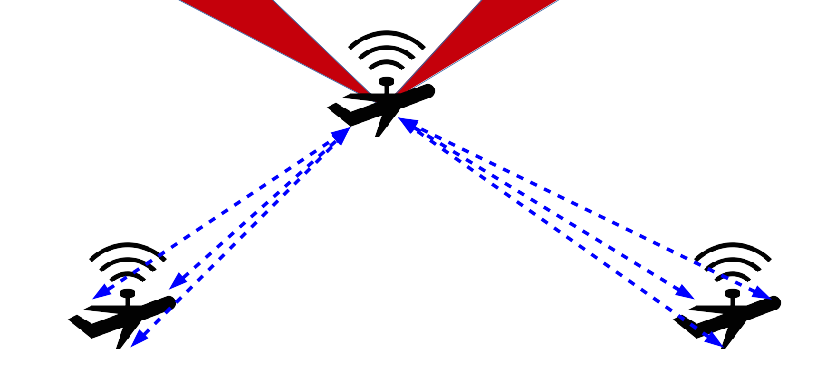
\includegraphics[width=0.8\textwidth]{images/attack4.png}
  \caption{Using the information of multiple drones to check distances hinders the task of a possible attacker, as multiple signals have to be relayed properly.}
  \label{fig:attackexample4}
\end{figure}

This trade-off between communication load and security is the only restriction on this solution. Different applications will have different needs, and the delay between messages has to be considered as well (a node A can report to B the position of a third node C on a given time, but B must consider the delay of the transmission with A when checking the received data).\\










\section{Conclusions}
\label{sec:conclusions}

From the results on the first research question we can conclude that, even though the explored scenarios are only a subject of investigation right now, and have no commercial use at the moment of writing this document, both autonomous cars and drones will surely be amongst the most important developments in the upcoming years. This makes the vulnerabilities on distance-bounding protocols a latent problem.\\

As systems like the drone delivery and automated cars are not yet available to the open public, is it difficult to foresee what systems and protocols these platforms will use. However, in this document the usefulness of including distance-bounding protocols on them has been explained, focusing on the consequences distance-amplification attacks might have on them.\\

Multiple solutions to these distance-amplification attacks have been proposed and discussed. Even though upper-distance bound cannot be solved as lower-distance bound by using limitations on the information travelling speed, the proposed solutions noticeably decrease the chances of a malicious party successfully attacking the protocol.\\




















\section{Acknowledgements}
\label{sec:acknowledgements}

We would like to thank Jordi van den Breekel and Paul van Iterson, supervisors of this project at KPMG, for their support over the course of this project. In a similar way, we would also like to thank Jaap van Ginkel and Arno Bakker, staff at the System and Network Engineering MSc, for their insight and guidance.\\







\printbibliography


%%% APPENDIX

\end{document}
